\documentclass[11pt,landscape]{article}
\usepackage{multicol}
\usepackage{calc}
\usepackage{ifthen}
\usepackage[landscape]{geometry}
\usepackage{hyperref}
\usepackage{lipsum}

\ifthenelse{\lengthtest { \paperwidth = 11in}}
	{ \geometry{top=.5in,left=.5in,right=.5in,bottom=.5in} }
	{\ifthenelse{ \lengthtest{ \paperwidth = 297mm}}
		{\geometry{top=1cm,left=1cm,right=1cm,bottom=1cm} }
		{\geometry{top=1cm,left=1cm,right=1cm,bottom=1cm} }
	}

% Turn off header and footer
\pagestyle{empty}
\usepackage{amsmath}

% Redefine section commands to use less space
\makeatletter
\renewcommand{\section}{\@startsection{section}{1}{0mm}%
                                {-1ex plus -.5ex minus -.2ex}%
                                {0.5ex plus .2ex}%x
                                {\normalfont\large\bfseries}}
\renewcommand{\subsection}{\@startsection{subsection}{2}{0mm}%
                                {-1explus -.5ex minus -.2ex}%
                                {0.5ex plus .2ex}%
                                {\normalfont\normalsize\bfseries}}
\renewcommand{\subsubsection}{\@startsection{subsubsection}{3}{0mm}%
                                {-1ex plus -.5ex minus -.2ex}%
                                {1ex plus .2ex}%
                                {\normalfont\small\bfseries}}
\makeatother

% Define BibTeX command
\def\BibTeX{{\rm B\kern-.05em{\sc i\kern-.025em b}\kern-.08em
    T\kern-.1667em\lower.7ex\hbox{E}\kern-.125emX}}

% Don't print section numbers
\setcounter{secnumdepth}{0}
\usepackage{circuitikz}

\setlength{\parindent}{0pt}
\setlength{\parskip}{0pt plus 0.5ex}
\usepackage{karnaugh-map}

% -----------------------------------------------------------------------

\begin{document}

\raggedright
\footnotesize
\begin{multicols*}{4}

% multicol parameters
% These lengths are set only within the two main columns
%\setlength{\columnseprule}{0.25pt}
\setlength{\premulticols}{1pt}
\setlength{\postmulticols}{1pt}
\setlength{\multicolsep}{1pt}
\setlength{\columnsep}{2pt}

\begin{center}
     \Large{\textbf{ECE253 Final Cheatsheet}}\\
     \small{\textit{Author: your mother}} \\
\end{center}
\subsection{RS Latch}
Sequential circuits depend on sequence of inputs. A \textbf{SR Latch} are cross-coupled \verb!NOR! gates.
% \begin{center}
    {
    \begin{multicols}{2}
        \begin{center}
            \begin{circuitikz} \draw
                (0,2) node[nor port] (NOR1) {}
                (1,2) node[anchor=east] {Q}
                (1,0) node[anchor=east] {$\overline{Q}$}
                (0,0) node[nor port] (NOR2) {}
                (NOR1.in 1) node[anchor=east] {R}
                (NOR2.in 2) node[anchor=east] {S}
                (NOR1.out) -- ++(0,-0.5) -- ($(NOR2.in 1) +(0,0.5)$) -- (NOR2.in 1)
                (NOR2.out) -- ++(0,+0.5) -- ($(NOR1.in 2) +(0,-0.5)$)--(NOR1.in 2)
                ;\end{circuitikz}
        \end{center}
        \begin{center}
            \begin{tabular}{c|c|c|c}
                S & R & Q & $\overline{Q}$ \\ \hline
                0 & 0 & 0/1 & 1/0 \\
                 0 & 1 & 0 & 1 \\
                1 & 0 & 1 & 0 \\
                1 & 1 & 0 & 0
           \end{tabular}
        \end{center}
        \vspace{-2mm}
        \scriptsize When $S=R=0$, it stores the last $Q$ value. In practice, we should not have $S=R=1$.
    \end{multicols}
}
\subsection{Gated D Latch and Clock Signal}
{
    \begin{multicols}{2}
        \begin{center}
            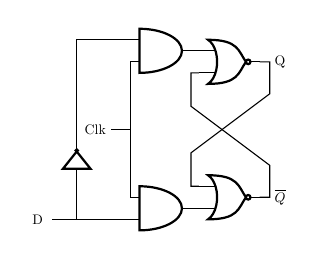
\begin{tikzpicture}[scale=0.5, transform shape]
                % Draw and gates
                \node[and port] (and1) at (0,2) {};
                \node[and port] (and2) at (0,-2) {};
                % Draw nor gates
                \draw (and1.out) -- ++(0.2,0) node
                [
                    nor port,
                    anchor=in 1
                ] (nor1) {};
                 
                \draw (and2.out) -- ++(0.2,0) node
                [
                    nor port,
                    anchor=in 2
                ] (nor2) {};
                 
                \draw (nor1.in 2) -| ++ (-0.2,-0.85) -- ++(2,-1.5) coordinate(a) |- (nor2.out);
                \draw (nor2.in 1) -| ++ (-0.2,0.85) -- ++(2,1.5) |- (nor1.out);
                % Clock
                \draw (and1.in 2) -- (and2.in 1)node[midway](clk){};
                \draw (clk.center) -- ++(-0.5,0) node[left]{Clk};
                % Output labels
                \draw (nor1.out -| a) node[right]{Q};
                \draw (nor2.out -| a) node[right]{$\overline{Q}$};
                \draw (and2.in 2) -- ++(-2,0) coordinate(a2) node[left=0.1cm]{D};
                % Not port
                \node
                [
                    not port,
                    rotate=90,
                    scale=0.5,
                ](not) at (-2.75,-0.75){};
                 
                \draw (not.in) |- (a2) (not.out) |- (and1.in 1)  ;
                 
                \end{tikzpicture}
        \end{center}
        \begin{center}
            \begin{tabular}{c|c}
                Clk & $Q(t+1)$ \\ \hline
                0 & Q(t) \\
                1 & D
           \end{tabular}
        \end{center}
        \vspace{-3mm}
    \end{multicols}
}
% \end{center}
\subsection{D Flip Flops}
Consists of two gated D latches, connected in series and both connected to the same clock. However, clock input for the first D latch is inverted. When the clock rises up, $Q$ stores value of $D$.
\subsection{T Flip Flops}
\begin{multicols}{2}
    \includegraphics[width=1.1\linewidth]{figures/T.png}
    \begin{center}
        \begin{tabular}{c|c|c}
        clk & $Q(t+1)$ \\ \hline
        $\uparrow$ & \verb!T^Q(t)!
   \end{tabular}
    \end{center}
\end{multicols}
\subsection{SystemVerilog}
\subsubsection{Logic Operators}
\begin{center}
    \begin{tabular}{c|c||c|c}
        \verb!bitwise AND! & \verb!&! &
        \verb!bitwise OR! & \verb!|! \\ \hline
        \verb!bitwise NAND! & \verb!~&! &
        \verb!bitwise NOR! & \verb!~!!  \\ \hline
        \verb!bitwise XOR! & \verb!^! &
        \verb!bitwise XNOR! & \verb!~^! \\ \hline
        \verb!logical negation! & \verb!!! &
        \verb!bitwise negation! & \verb!~! \\ \hline 
        \verb!concatenation! & \verb!{}! &
        \verb!replication! & \verb!{{}}! 
    \end{tabular}
\end{center}
\begin{itemize}
    \item \verb!reduction! operators are put at the start and output a scalar.
    \item \verb!bitwise! operators
    \item \verb!blocking assignment =!: executed in the order they are specified.
    \item \verb!Nonblock assignments <=! executed in parallel.
    \item Use \verb!logic! instead of \verb!reg/wire! (4-state type)
    \item Use \verb!always_comb! for combinational, \verb!always_ff! for sequential logic
\end{itemize}

\subsubsection{Case Statements}
\begin{verbatim}
module mux(
    input logic [2:0] MuxSelect,
    input logic [4:0] Input,
    output logic Out
);
    always_comb begin
        case (MuxSelect)
            3'b000: Out = Input[0];
            // ...
            3'b100: Out = Input[4];
            default: Out = 1'bx;
        endcase
    end
endmodule
\end{verbatim}
\subsubsection{Half Adder}
\begin{verbatim}
module HA(
    input logic x, y,
    output logic s, c
);
    assign s = x ^ y;
    assign c = x & y;
endmodule
\end{verbatim}
\subsubsection{Full Adder}
\begin{verbatim}
module FA(
    input logic a, b, c_in,
    output logic s_out, c_out
);
    logic w1, w2, w3;
    HA u0(.x(a), .y(b), .s(w1), .c(w2));
    HA u1(.x(c_in), .y(w1), .s(s_out), .c(w3));
    assign c_out = w2 | w3;
endmodule
\end{verbatim}
\subsection{D Flip Flop}
\begin{verbatim}
module D_ff(
    input logic D, clk,
    output logic Q
);
    always_ff @(posedge clk)
        Q <= D;
endmodule
\end{verbatim}
\subsection{T Flip Flops}
\begin{verbatim}
module t_ff(
    input logic Clock, Clear_b, T,
    output logic Q
);
    always_ff @(posedge Clock, negedge Clear_b) begin
        if (Clear_b == 1'b0)
            Q <= 1'b0;
        else
            Q <= T ^ Q;
    end
endmodule
\end{verbatim}
\subsection{Registers}
\begin{verbatim}
module reg8(
    input logic clk,
    input logic [7:0] D,
    output logic [7:0] Q
);
    always_ff @(posedge clk)
        Q <= D;
endmodule
\end{verbatim}
\subsection{ModelSim Do Files}
\begin{verbatim}
# set working dir, where compiled verilog goes
vlib work
# compile all verilog modules in mux.v to working
# dir could also have multiple verilog files
vlog mux.v
#load simulation using mux as the
# top level simulation module
vsim mux
#log signals and add signals to waveform window
log {/*}
# add wave {/*} would add all items in
# top level simulation module
add wave {/*}
# set input values using the force command
# signal names need to be in {} brackets
force {SW[0]} 0
force {SW[1]} 0
run 10ns
\end{verbatim}
\textbf{ModelSim and Other Lab Things}
\begin{itemize}
    \item FGPA: Field Programmable Gate Array
    \item To repeat signals, use this syntax:
    \begin{verbatim}
force {MuxSelect[2]} 0 0ns, 1 {4ns} -r 8ns
    \end{verbatim}
    \vspace{-4mm}
    which starts at $0$ at 0ns, $1$ at 4ns, and repeats every $8$ ns.
    \item On the \verb!DE1-SoC! board, hex thing is red if $0$ and white if $1$.
\end{itemize}
\subsection{Frequency Dividers}
\begin{itemize}
    \item To half the frequency, connect $\overline{Q}$ to $D$ on the same gated D latch.
    \item To quarter the frequency, connect $\overline{Q}$ to the clock of the next gated D latch (which is set up the same as the half frequency case).
    \item To reduce frequency by $2k$, connect $k$ D latches connected in series ($D$ to $Q$) and to the same clock. First $D$ is connected to last $\bar{Q}$. The last $Q$ will have a reduced frequency of $2k$.
\end{itemize}
\subsection{Resets}
\begin{itemize}
    \item Active High/Low: Resets when Signal is 1/0
    \item Synchronous High/Low: Resets during positive/negative edge
\end{itemize}
\section{Finite State Machines}
{\scriptsize
\textbf{Steps:} (1) State Diagram (2) State Table (3) State Assignment (4) State-Assigned Table (5) Synthesize Circuit

\textbf{State Encoding:} \textit{One-hot:} $n$ states = $n$ flip flops (A=0000001, B=0000010, ...). \textit{Binary:} $n$ states = $\lceil\log_2 n\rceil$ flip flops (000, 001, 010, ...).

\textbf{Synthesis:} Write $Y_n=f_n(y_1,\ldots,W)$, $z=g(y_1,\ldots)$. For each FF $i$: input=$Y_i$, output=$y_i$. Output branches to (1) $g$ for output $z$, (2) $f_n$ loops back to $Y_n$. FFs share clock/reset.
}
\subsection{FSM in SystemVerilog}
{\scriptsize
\begin{verbatim}
module FSM(input logic Clock, Resetn, w,
    output logic z, output logic [3:0] CurState);
logic [3:0] y_Q, Y_D;
typedef enum logic [3:0] {A=4'b0000, B=4'b0001,
    /*...*/ G=4'b0110} state_t;
always_comb begin
    case (y_Q)
        A: Y_D = w ? B : A;
        /*...*/
        G: Y_D = w ? C : A;
        default: Y_D = A;
    endcase
end
always_ff @(posedge Clock) begin
    if (!Resetn) y_Q <= A;
    else y_Q <= Y_D;
end
assign z = (y_Q == F) | (y_Q == G);
assign CurState = y_Q;
endmodule
\end{verbatim}
}
\section{RISC-V Assembly}
\subsection{Conditionals}
\vspace{-2mm}
{\scriptsize
RISC-V has no flags. Branch instructions: \verb!beq! (equal), \verb!bne! (not equal), \verb!blt/bge! (less/greater signed), \verb!bltu/bgeu! (unsigned). Set: \verb!slt!, \verb!slti!, \verb!sltu!, \verb!sltiu!.
}
\subsection{Interrupts}
\vspace{-2mm}
{\footnotesize
\begin{enumerate}\setlength\itemsep{-0.5em}
    \item Set \verb!mtvec! CSR (trap vector)
    \item Enable interrupts in \verb!mstatus! (MIE bit)
    \item Enable sources in \verb!mie! CSR
    \item Configure PLIC/CLIC
    \item Save context on trap entry
    \item Read \verb!mcause! CSR for cause
    \item Handle in ISR, clear PLIC pending bit
    \item Restore context, return with \verb!mret!
\end{enumerate}}
\section{RISC-V Assembly Example Code}
\subsection{Enabling Interrupts}
\vspace{-2mm}
{\scriptsize
\begin{verbatim}
li sp, 0x10000        # Initialize stack
la t0, trap_handler
csrw mtvec, t0        # Set trap vector
li t0, 0x8
csrs mstatus, t0      # Enable interrupts (MIE)
li t0, 0x800
csrs mie, t0          # Enable external int (MEIE)
li t0, 0xFF20058
li t1, 0b1001
sw t1, 0(t0)          # Enable key3, key0
\end{verbatim}}
\subsection{Check Cause of Interrupt}
\vspace{-2mm}
{\scriptsize
\begin{verbatim}
trap_handler:
    addi sp, sp, -32
    sw t0, 0(sp); sw t1, 4(sp); sw a0, 8(sp)
    sw a1, 12(sp); sw ra, 16(sp)
    csrr t0, mcause       # Read cause
    li t1, 0x8000000B
    bne t0, t1, error_trap
    jal ra, key_isr
    j exit_trap
error_trap:
    j error_trap
exit_trap:
    lw t0, 0(sp); lw t1, 4(sp); lw a0, 8(sp)
    lw a1, 12(sp); lw ra, 16(sp)
    addi sp, sp, 32
    mret
\end{verbatim}}
\subsection{ISR Subroutine}
\vspace{-2mm}
{\scriptsize
\begin{verbatim}
key_isr:
    addi sp, sp, -20
    sw t2, 0(sp); sw t3, 4(sp)
    sw t4, 8(sp); sw t5, 12(sp)
    la t5, CURR_VALUE
    lw t4, 0(t5)
    li t2, 0xFC20005C
    lw t3, 0(t2)
    li t0, 0b1000
    bne t3, t0, key0
    beq t4, zero, endisr
    addi t4, t4, -1
    sw t4, 0(t5)
    j endisr
key0:
    # code for key 0
endisr:
    lw t2, 0(sp); lw t3, 4(sp)
    lw t4, 8(sp); lw t5, 12(sp)
    addi sp, sp, 20
    ret
\end{verbatim}}
\subsection{Polled IO with Timer}
\vspace{-2mm}
{\scriptsize
\begin{verbatim}
.text
.globl _start
_start:
    li a0, 0xFFFEC600
    li a1, 200000000
    sw a1, 0(a0)
    li a1, 0b111
    sw a1, 8(a0)
    li s0, 0; li s1, 0; li s2, 0  # sec,min,hr
poll:
    lw a1, 12(a0)
    beq a1, zero, poll
    sw a1, 12(a0)
    addi s0, s0, 1
    li t0, 60
    bne s0, t0, poll
    li s0, 0
    addi s1, s1, 1
    bne s1, t0, poll
    li s1, 0
    addi s2, s2, 1
    li t0, 24
    bne s2, t0, poll
    li s2, 0
    j poll
\end{verbatim}}
\subsection{Exception Vector Table}
\vspace{-2mm}
{\scriptsize
\begin{verbatim}
.align 2
trap_vector:
    j trap_handler  # Direct: all to one handler
# Vectored: mtvec.MODE=1, base + 4*cause
# 0x00:Exception 0x04:Supervisor SW int
# 0x0C:Machine SW int 0x14:Supervisor timer
\end{verbatim}}
\subsection{Find Sum with Recursion}
\vspace{-2mm}
\begin{multicols}{2}
{\scriptsize
\begin{verbatim}
.globl _start
_start:
    li sp, 0x20000
    la s0, N
    lw a0, 0(s0)
    li a1, 0
    jal ra, findsum
    add a1, a1, a0
end: j end
findsum:
    addi sp, sp, -8
    sw a0, 0(sp); sw ra, 4(sp)
    li t0, 2
    blt a0, t0, return
    addi a0, a0, -1
    jal ra, findsum
    add a1, a1, a0
return:
    lw a0, 0(sp); lw ra, 4(sp)
    addi sp, sp, 8
    ret
.data
N: .word 5
\end{verbatim}}
\end{multicols}
\subsection{Fibonacci with Recursion}
\vspace{-2mm}
\begin{multicols}{2}
{\scriptsize
\begin{verbatim}
.data
N: .word 10
.text
.globl _start
_start:
    li sp, 0x20000
    la s0, N; lw a0, 0(s0)
    li a1, 0; li a2, 0
    jal ra, fib
end: j end
fib:
    addi sp, sp, -12
    sw a0, 0(sp); sw a2, 4(sp)
    sw ra, 8(sp)
    li t0, 2
    bge a0, t0, recur
    mv a1, a0
    lw a0, 0(sp); lw a2, 4(sp)
    lw ra, 8(sp)
    addi sp, sp, 12
    ret
recur:
    addi a0, a0, -1
    jal ra, fib
    mv a2, a1
    addi a0, a0, -1
    jal ra, fib
    add a1, a1, a2
    lw a0, 0(sp); lw a2, 4(sp)
    lw ra, 8(sp)
    addi sp, sp, 12
    ret
\end{verbatim}}
\end{multicols}
\section{Timing Analysis}
\subsection{Minimum Clock Period}
\vspace{-2mm}
$$T_{\min} = T_{su} + T_{CQ} + T_{logic}$$
$$F_{\max} = \frac{1}{T_{\min}}$$
\subsection{Hold Time Violation}
\vspace{-2mm}
For no hold time violation:
$$t_{hold} + t_{skew} \leq t_{CQ} + t_{logic}$$
where $t_{skew}$ is the minimum clock skew.
\end{multicols*}
\end{document}
